\chapter{Background Literature}
\label{BackgroundLit}


\section{Dementia and HCI}
\label{BL:DementiaHCI}
Over the last 40 years, researchers and care practitioners have seen our understanding of dementia evolve to position and represent the person with dementia in several ways. What was once a bio-medical stance has gradually moved towards one that considers the socio-political and individual experiences of dementia \citep{bellass_broadening_2019} . In the early years of dementia research, the biomedical view, dementia was viewed through its neurodegenerative condition, emphasising the person's abilities, memory, judgement and communication. Recognising these characteristics of dementia led to an awareness of strain on care partners towards policymakers, improvements in identifying and diagnosing dementia, and the development of medication to reduce symptoms of dementia \citep{doi:10.1080/13607863.2019.1693968}. Moreover, given that there are still no known treatments to stop the progression of dementia, there has been significant work and research funding into understanding the causes of the neurodegenerative condition \citep{bature_signs_2017}.

However, several negative consequences arose from such a biomedical lens that has had significant social ramifications on people with dementia. First, the biomedical view promotes a view of 'loss of self' \citep{ryan_dementia_2009}. Early work by \cite{cohen_loss_1986} believed that people living with dementia \textit{"must eventually come to terms with…the complete loss of self"}. Views of dementia that see it as a state of deficiency, often place the person living with dementia as a passive \textit{'patient'} where the condition is looked at being treated rather than understood. If acted upon, design and research do very little to aid the agency or the need for a continued sense of purpose and belonging \citep{hampson_dementia:_2016}. Second, as dementia progresses, it often adds conflict between their surroundings as they become unfamiliar, and in turn, causes difficulties coexisting in places with others, such as a family home or a workplace \citep{langdon_making_2007}. Finally, As we live in a society that places great value on cognitive ability, many believe that people with dementia are poor at social contact, which then prohibits many from interacting with people with dementia at all \citep{killick_communication_2001}.

From the early 90's, researchers began to contest the limitations of the biomedical stance by highlighting that the quality of life of the person with dementia is determined not only by neuropathology but also by how they are perceived in society, personal history, and interactions and desires \citep{o2007personhood}. There is growing literature indicating that an approach to care that supports inclusion, recognition, trust, and the individual's personhood may delay or reduce several negative consequences that may develop with dementia. Tom Kitwood, one of the more prominent researchers to tackle the biomedical view, defined the personhood of the person with dementia as \textit{"the standing or status that is bestowed upon one human being, by others, in the context of relationship and social being"} \citep[pg.8]{kitwood1997dementia}. Instead of seeing the person with dementia by their disease, Kitwood challenged this by centring the personhood of the person with dementia by personalising care, paying attention to the individual's relationships, and maintaining decision-making by acknowledging the person's abilities. While I describe the potential limitations of personhood in the later stages of this literature review, the concept of personhood has promoted necessary changes to dementia research and practice. For instance, the approach has brought forth the sharing of people's experiences with dementia that has redefined how we speak and involve people with dementia in research. Furthermore, the focus on lived experiences, has not only demonstrated the importance of individuality in care and when working with people living with dementia but has created a cultural and positive change towards those who have recently been diagnosed with dementia and began to address 'dementia worry' \citep{kessler_dementia_2012}.

An integral part of HCI work builds on personhood approaches where design and technology advancements have moved towards improving quality of life, supporting inclusion, evoking emotion, and engagement through creativity to help foster heightening subjective wellbeing, maintaining skills, and providing social engagement. While many creatively oriented technologies have relied on the person's ability to articulate past events or configure dementia as a series of problems, as researchers have moved toward the inclusion of the voices of people living with dementia, recent HCI research has similarly begun to question how to position people with dementia in the designing of technology appropriately. With this in mind, the following subsections review dementia-HCI literature that investigates the type of technologies, design, and participatory approaches researchers use in the domain.
% Add something here making it very clear what the nxt section is. Reviewing the literature -- highlight the current state of HCI literature + potential challenges / themes that the PhD will explore

\subsection{Moving to a user-centered approach}
\label{BL:Tech}
Within HCI, early work in dementia focused on the role of assistive (or enabling) technology to support independent living for people with dementia. \cite{bharucha2009intelligent} review of assistive technology applications highlight an array of different sensors and devices built to compensate for physical and cognitive deficits of people with dementia. For instance, the authors highlight one device, in particular, GPS, to tackle the problem of 'wandering'. The term wandering derives from categorising particular 'behaviours' in people with dementia where individuals may get lost or forget where they were going. While walking is beneficial to the person with dementia, the action of 'wandering' has often been associated with potential harm and emotional stress for the person with dementia and their care partners (Robinson - balancing rights and risks). As \cite{bharucha2009intelligent} highlight, these early studies focusing on 'problems' caused by dementia, would be guided by family and professional care staff instead of people with dementia. Similarly, early work in care home architecture \citep{torrington2006has}, care processes \citep{rabins2006practical}, and creative therapy \citep{schmitt2006creative} prioritised those without dementia in the development processes with the potential of people with dementia invited in the evaluation phases of development. This has resulted in prior products and services failing to represent the desires and needs of people with dementia causing a lack of uptake and ownership of technology design \citep{gibson2019personalisation}. 

Given the overwhelming focus on technology that considers how to 'fix' challenges, researchers have introduced user-centred, participatory design methods that have brought attention to promoting personhood through the technologies we are designing. For instance, \cite{robinson2009keeping} ran a series of user-centred design sessions with people with dementia and their carers to design and develop a set of prototypes to facilitate independence for the person with dementia and centre the voices of people with dementia in the design process. The authors' findings highlight opportunities for involving people with dementia in technology's design and curation stages. The technology customisation was well received and necessary to be tailored to the person with dementia's assistive needs. However, while this work stresses that there is no one-size-fits-all approach when designing assistive technologies, researchers need to consider how we may design mass customisation techniques to deliver commercial personalised devices. Furthermore, \cite{robinson2009keeping} remark that adoption will require the support of user-friendly interfaces for carers to ensure the person with dementia use the assistive technology. 

\cite{wallace_enabling_2012-1wallace_design-led_2013} extends the user-centred approach by turning to a more experiential and relational approach known as experience-centred design (ECD). Through this approach, ECD focuses on \textit{"an understanding of individuals, their concerns, desires, aspirations, values, and experiences"} \citep{morrissey_value_2017} constructed by dialogue, storytelling, and reflection. In Wallace's paper - A Design-led Inquiry into Personhood in Dementia \citep{wallace_design-led_2013}, the author's works closely with a married couple (John and Gillian), where the wife had recently been diagnosed with dementia, to design pieces of digital jewellery to support Gillian's personhood. To involve and empathically engage the couple in the design process of the jewellery, the study was carried out as a piece of research through design (RTD). RTD is a way of doing research, which is the practice of design used to address wicked problems that entail a sense of complexity and have no current solution. The approach seeks to address the problem within its current situation \citep{zimmerman_research_2007}. It is generally acknowledged to involve end-users within the design process to address and reflect on, problems within the associated design space. Through the output of RTD being the creation of digitally-mediated experiences, the interactions and design decisions provided \cite{wallace_design-led_2013} insights into the experiences of the couple in order to keep the experience alive in the digital jewellery. For instance, the Self Tree probe consists of oval lockets on a small branch, which emphasises Gillian's rich relationships that provides \textit{"aspects of who she is, how other people value her, and how this network of individuals is connected through her"}.

These sorts of studies that pay attention to the experience of dementia within HCI, often lead to 'unfinished' objects but rather unpacks the creativity of the design process that ultimately reveals how people with dementia may intend to use technology that may be the polar opposite of the designer's original intentions. While Wallace highlights the value in this approach to provide insights and understandings into the experiences of people with dementia, exploratory studies that build technology may fall short in supporting the longevity of the technology resulting in complexities for the participants in the long term. Returning to \cite{robinson2009keeping}, the authors echo similar concerns where people with dementia "may become distressed if a prototype does not work". \cite{meurer_designing_2018} discusses the problems of innovation and its impact on sustainability. 

The drive to create exploratory research puts pressure on technology solutions that may not be appropriate for the community. However, research may be ill-judged on funding for continued support after the project ends. Researchers can still fall into technology-focused ethical difficulties even when the research may collaborate with large technology corporations. \cite{vines_our_2017} describes frustrations while using Google Glass in its beta stages, where participants would encounter many breaking bugs. These bugs ranged from poor battery life, to Google Glass updating itself while in use in spite of participants' wishes to the contrary. With these additional complexities, there are opportunities to consider ways to counteract the robustness and longevity of technology when the project ends. To do this, perhaps research may focus on building genuine connections with the participants that mirrors Wallace's work or perhaps building communities of people with dementia, designers and developers who may support the longevity of the technology. To dive deeper into understanding participation and relationship building in dementia-HCI research, the following two subsections explore a) the type of participation in the different phases of development and b) the value in relationship building between researchers and people with dementia.
%finishing this bit to be more focused on the below

\subsection{The stages of participation in technology development}
\label{BL:StagesofTech}

\begin{figure}[htp]
    \centering
    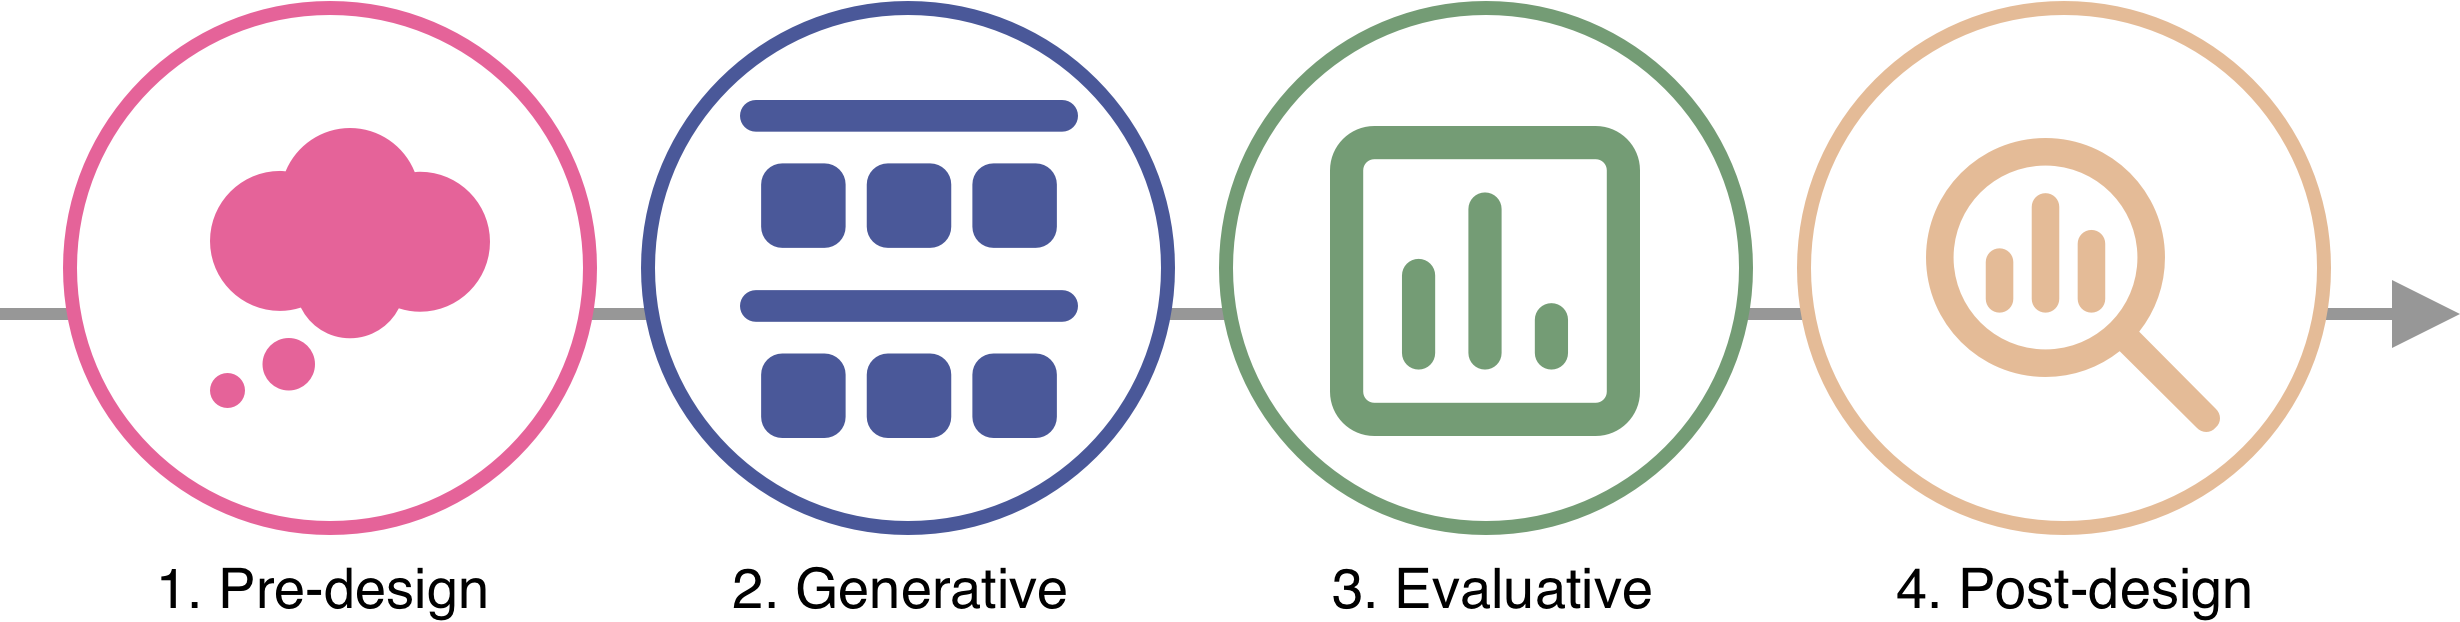
\includegraphics[width=0.8\linewidth]{Images/ChapterTwo/PhasesOfTech.png}
    \caption{Four phases of tech development \citep{suijkerbuijk_active_2019}}
    \label{fig:PhasesOfTech}
\end{figure}
In a recent systematic review of developing supportive technologies for and with people with dementia, \cite{suijkerbuijk_active_2019} categorise technology development into four phases: pre-design, generative, evaluative, and post-design (seen in fig \ref{fig:PhasesOfTech}). In this subsection, I dive into a series of dementia-HCI studies that involve people with dementia in the different stages of development. This sub-section aims to focus on the type of people with dementia who are included (or instead excluded), alongside the type of methods and approaches researchers adopt to involve the voices of people with dementia.

\subsubsection{Pre-design}
\label{BL:Pre-Design}




